\documentclass[12pt,onecolumn]{IEEEtran}
\usepackage{graphicx}
\usepackage{booktabs}
\usepackage{hyperref}
\usepackage{amsmath}

\title{Reproducible Drug Safety Signal Detection on Public FAERS Data}
\author{Saif Mohammed\\Seattle University}

\begin{document}
\maketitle

\begin{abstract}
We present an open-source pharmacovigilance workflow for reproducing
disproportionality-based drug safety signal detection on public FDA Adverse
Event Reporting System (FAERS) data. The pipeline implements PRR and ROR signal
detection, robust artifact filtering, BCPNN IC025 and simplified EBGM/EB05
baselines, XGBoost ranking, and historical warning backtesting. On the current
2020-12-31 cutoff validation artifact, the workflow detects 1 of 7 post-cutoff
FDA warning pairs: UPADACITINIB--MYOCARDIAL INFARCTION, first crossing the
signal threshold 519 days (17.3 months) before the reference FDA warning date.
The contribution is not a clinical decision support claim; it is a reproducible
workflow and an empirical characterization of the false-positive-dominant nature
of naive FAERS disproportionality analysis.
\end{abstract}

\section{Introduction}
Spontaneous adverse-event reporting systems are widely used for post-marketing
drug safety surveillance. Public FAERS data enables reproducible research, but
naive disproportionality analysis produces many artifacts. This work builds a
local, zero-cost pipeline for signal detection and backtesting.

\section{Background}
The 2x2 contingency table for drug $D$ and reaction $R$ contains observed
co-report count $a$, drug-without-reaction count $b$, reaction-without-drug
count $c$, and all-other count $d$. We evaluate PRR, ROR, BCPNN IC025, and
simplified EBGM/EB05.

\section{Related Work}
Classical disproportionality methods include PRR \cite{evans2001prr}, ROR
\cite{vanpuijenbroek2002ror}, BCPNN \cite{bate1998bcpnn}, and MGPS
\cite{dumouchel1999mgps}. Reviews of spontaneous-reporting data mining discuss
the strengths and limitations of these methods \cite{hauben2009review,
sakaeda2013faers,noren2013shrinkage}.

\section{Methods}
The pipeline downloads FAERS quarterly data, parses nested JSON into flattened
drug/reaction observations, computes PRR/ROR in PySpark and Hive/HQL, trains an
XGBoost ranking model, and stores dashboard-ready outputs. Robust filtering
requires minimum case count, minimum country-count source proxy, seriousness
ratio, bounded PRR/ROR, and non-negative chi-square.

\begin{figure}[h]
\centering
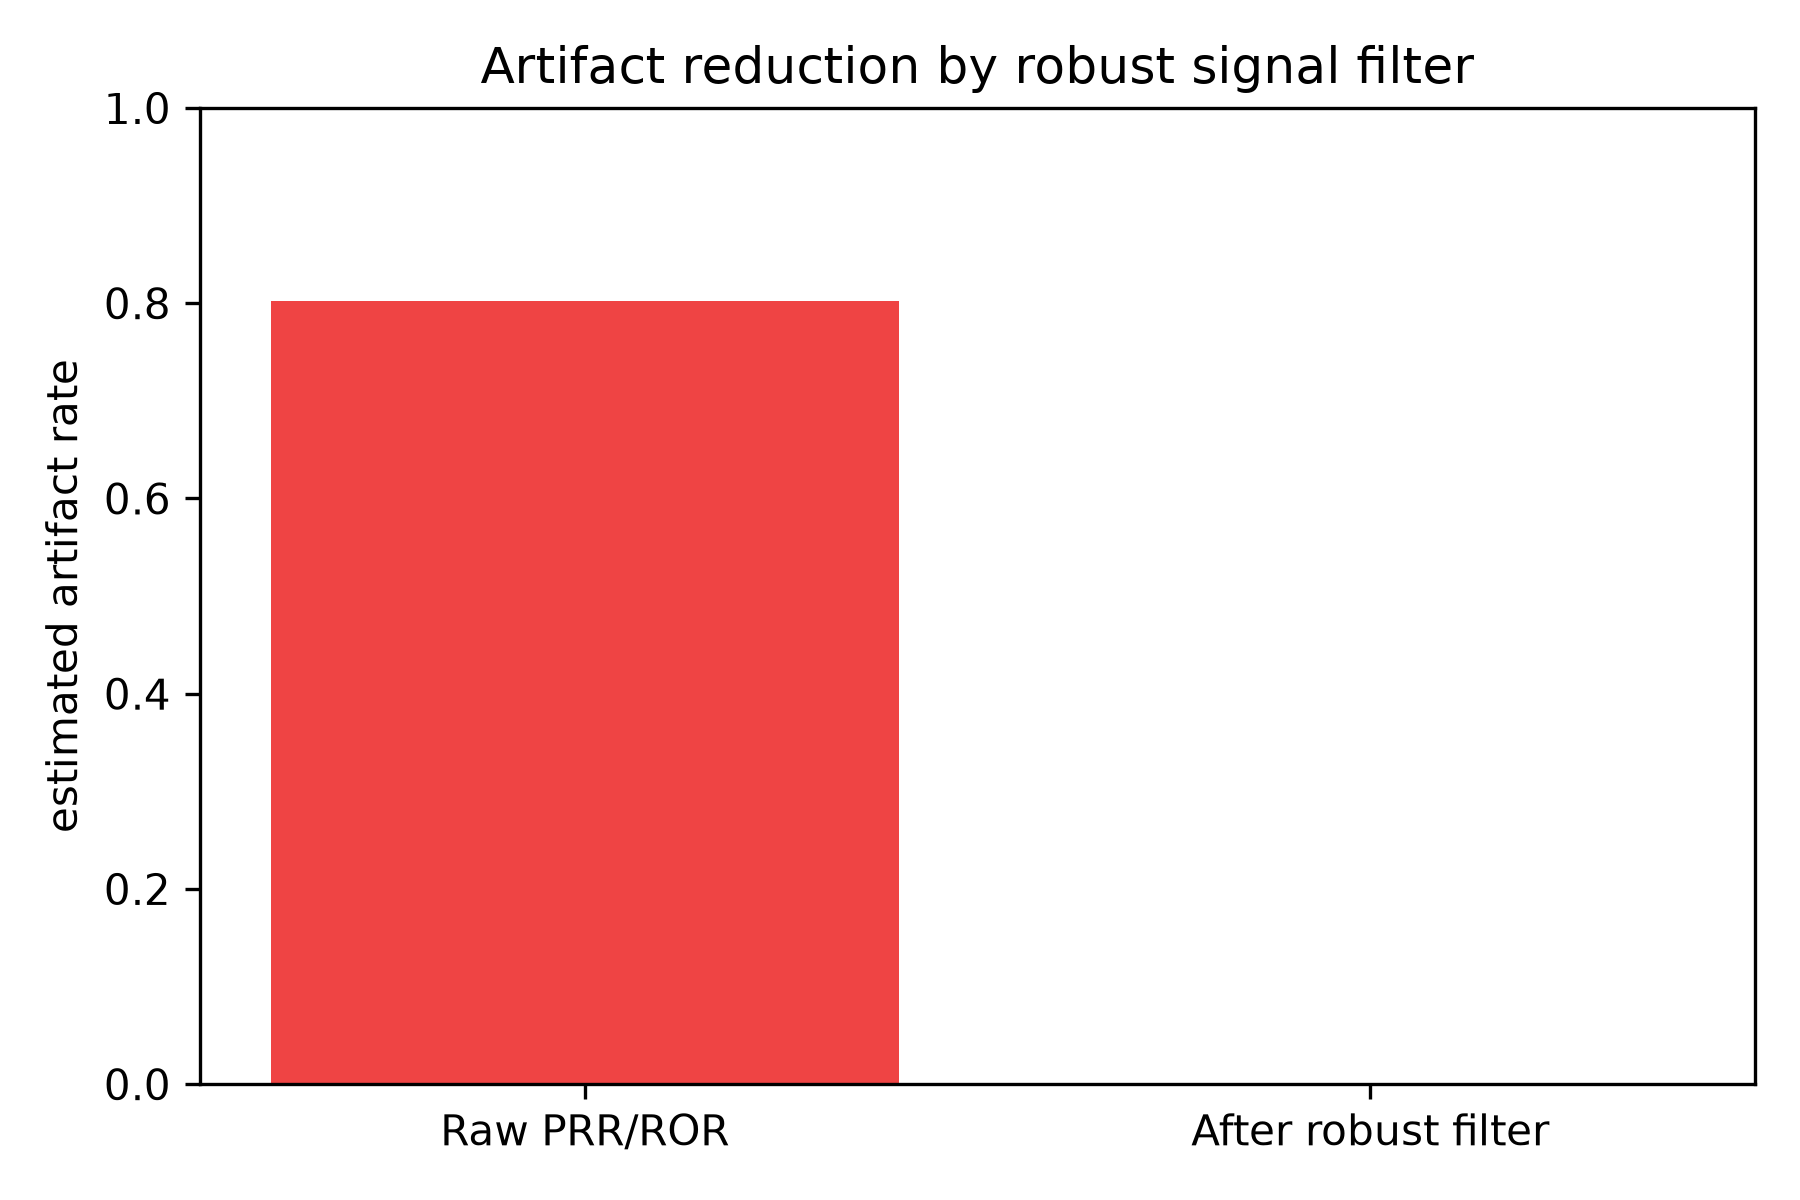
\includegraphics[width=0.95\linewidth]{../docs/figures/artifact_rate_before_after.png}
\caption{Estimated artifact rate before and after robust signal filtering.}
\end{figure}

\section{Experimental Setup}
Experiments run locally on macOS Apple Silicon with Python 3.11. The Docker
stack smoke test validates HDFS, Hive, PostgreSQL, API, and Streamlit services
on a small real Parquet sample. Full feature generation runs locally with
PySpark.

\section{Results}
\begin{tabular}{lllllll}
\toprule
cutoff & method & warnings & recall & recall_95ci & precision & lead_days \\
\midrule
2018-12-31 & \textbf{future warnings} & \textbf{11} &  &  &  &  \\
2018-12-31 & PRR/ROR & 2/11 & 0.182 & [0.00, 0.45] & 4.0e-06 & 566 \\
2018-12-31 & Robust PRR/ROR & 2/11 & 0.182 & [0.00, 0.45] & 2.0e-05 & 566 \\
2018-12-31 & BCPNN IC025 & 3/11 & 0.273 & [0.00, 0.55] & 2.4e-05 & 566 \\
2018-12-31 & EBGM/EB05 & 2/11 & 0.182 & [0.00, 0.45] & 9.8e-06 & 566 \\
2018-12-31 & XGBoost >= 0.5 & 2/11 & 0.182 & [0.00, 0.45] & 1.8e-05 & 566 \\
2019-12-31 & \textbf{future warnings} & \textbf{10} &  &  &  &  \\
2019-12-31 & PRR/ROR & 2/10 & 0.200 & [0.00, 0.50] & 4.0e-06 & 566 \\
2019-12-31 & Robust PRR/ROR & 2/10 & 0.200 & [0.00, 0.50] & 2.0e-05 & 566 \\
2019-12-31 & BCPNN IC025 & 3/10 & 0.300 & [0.00, 0.60] & 2.4e-05 & 566 \\
2019-12-31 & EBGM/EB05 & 2/10 & 0.200 & [0.00, 0.50] & 9.8e-06 & 566 \\
2019-12-31 & XGBoost >= 0.5 & 2/10 & 0.200 & [0.00, 0.50] & 1.8e-05 & 566 \\
2020-12-31 & \textbf{future warnings} & \textbf{7} &  &  &  &  \\
2020-12-31 & PRR/ROR & 1/7 & 0.143 & [0.00, 0.43] & 2.0e-06 & 519 \\
2020-12-31 & Robust PRR/ROR & 1/7 & 0.143 & [0.00, 0.43] & 1.0e-05 & 519 \\
2020-12-31 & BCPNN IC025 & 2/7 & 0.286 & [0.00, 0.71] & 1.6e-05 & 519 \\
2020-12-31 & EBGM/EB05 & 1/7 & 0.143 & [0.00, 0.43] & 4.9e-06 & 519 \\
2020-12-31 & XGBoost >= 0.5 & 1/7 & 0.143 & [0.00, 0.43] & 9.0e-06 & 519 \\
2021-12-31 & \textbf{future warnings} & \textbf{3} &  &  &  &  \\
2021-12-31 & PRR/ROR & 0/3 & 0.000 & [0.00, 0.00] & 0.0e+00 &  \\
2021-12-31 & Robust PRR/ROR & 0/3 & 0.000 & [0.00, 0.00] & 0.0e+00 &  \\
2021-12-31 & BCPNN IC025 & 0/3 & 0.000 & [0.00, 0.00] & 0.0e+00 &  \\
2021-12-31 & EBGM/EB05 & 0/3 & 0.000 & [0.00, 0.00] & 0.0e+00 &  \\
2021-12-31 & XGBoost >= 0.5 & 0/3 & 0.000 & [0.00, 0.00] & 0.0e+00 &  \\
\bottomrule
\end{tabular}


\begin{tabular}{llllrll}
\toprule
drug & reaction & warning date & signal first detected & days early & months early & lead time basis \\
\midrule
UPADACITINIB & MYOCARDIAL INFARCTION & 2021-09-01 & 2020-03-31 & 519 & 17.3 & signal\_first\_detected\_date \\
\bottomrule
\end{tabular}


\section{Discussion}
% TODO: Discuss why false positives dominate public FAERS signal detection,
% confounding by indication, and why robust filtering improves interpretability.

\section{Limitations}
The warning reference set is small and hand-curated. FAERS reports do not prove
causality. Public FAERS extracts do not expose a clean reporter-source ID, so
country count is used as a conservative source-diversity proxy. The current
validated result catches only 1 of 7 post-cutoff warnings for the 2020 cutoff.

\section{Reproducibility}
All code is available in the accompanying repository. Generated feature Parquet
and raw FAERS files are intentionally excluded from Git. See
\texttt{docs/REPRODUCIBILITY.md}.

\section{Conclusion}
% TODO: Summarize the reproducible workflow contribution and future work:
% stronger ground truth, MedDRA grouping, and richer empirical Bayes baselines.

\bibliographystyle{IEEEtran}
\bibliography{references}
\end{document}

